\chapter{Contexte / Environnement}
\label{chap:premierchapitre}

Dans ce chapitre, nous allons présenter l'entreprise Sopra Steria, sa structure, l'agence 151 du secteur public, ainsi que le client auquel nos développements sont destinés : la CNAM.

\section{Organisation du groupe}

Sopra Steria est née de la fusion en 2014 de deux des plus anciennes Entreprises de Services du Numérique françaises : Sopra et Steria, fondées respectivement en 1968 et 1969 et marquées toutes deux par un fort esprit entrepreneurial ainsi qu'un grand sens de l’engagement collectif au service de ses clients.

\subsection{Sopra Steria dans le monde}

Le Groupe s'affirme comme un des leaders européens de la transformation numérique.

Suite à cette fusion le groupe compte près de 42 000 collaborateurs répartis dans plus de 20 pays et a réalisé un chiffre d’affaire de 3,8 milliards d’euros en 2017.

\begin{figure}[!h]
\centering

\includegraphics[width=0.8\textwidth]{images/chiffres_cles2017.jpg}
\caption{Sopra Steria : Leader européen de la transformation numérique}
\end{figure}

Sopra Steria devient alors l'un des leader Européen de la transformation numérique.

\begin{figure}[!h]
\centering
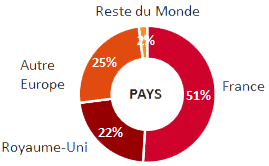
\includegraphics[width=0.5\textwidth]{images/payssoprasteria.png}
\caption{Sopra Steria : Répartition de l'activité en fonction des pays}
\end{figure}

Cette fusion a pris grâce à une forte complémentarité entre les deux entreprises : Sopra Group étant très implanté en France et peu à l'international et Steria étant une entreprise reconnue à l'international, notamment en Europe.

L’entreprise intervient dans de nombreux secteurs et domaines d’activité :

\begin{figure}[!h]
\centering
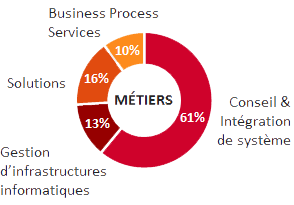
\includegraphics[width=0.5\textwidth]{images/metier_soprasteria.png}
\caption{Sopra Steria : Répartition des activités en fonction des métiers}
\end{figure}

\subsection{Les différents secteurs d'activités}

La figure ci-dessous illustre la première division s’effectuant par secteur d’activité :

\begin{figure}[!h]
\centering
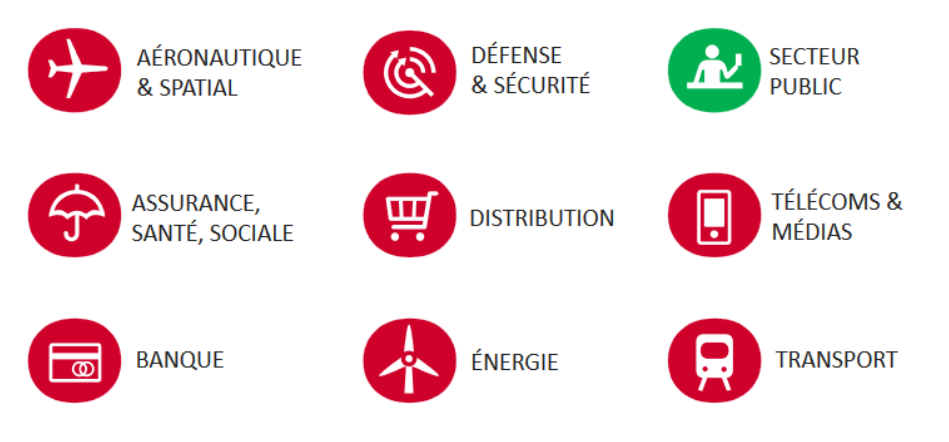
\includegraphics[width=0.8\textwidth]{images/secteurActivite.png}
\caption{Sopra Steria : Secteurs d'activités}
\end{figure}

Le Secteur Public est le marché majoritaire chez Sopra Steria Group puisqu’il représente 25\% de son chiffre d’affaires. La Business Unit(BU) du Secteur public est répartie sur 4 agences :  

\begin{itemize}
    \item Santé, Social, Emploi : Agence 151 (Sécurité sociale, Pôle emploi, CNAM…), 
    \item Recherche Enseignement : Agence 152 (Ministère Éducation Nationale, …), 
    \item Administration Centrale : Agence 156 (Mairie de Paris, DGFIP, ONP …), 
    \item Conseil : Agence 155 (Clients transverses à toute la BU). 
\end{itemize}

Pour ma part, je travaille au sein de l’agence 151, pour le compte de la CNAM.

Au sein d'un même secteur d'activité, l'entreprise est divisée en agences qui fonctionnent comme des entreprises autonomes. Elles ont chacun un directeur d'agence disposant d'un grand pouvoir décisionnel au sein de son agence. Une agence prend en charge de nombreux projets. Dans notre cas, l'agence 151 gère les missions relevant du domaine de la Santé, du Social et de l’Emploi.
Voir ci-dessous la division au sein du secteur public.

\begin{figure}[!h]
\centering
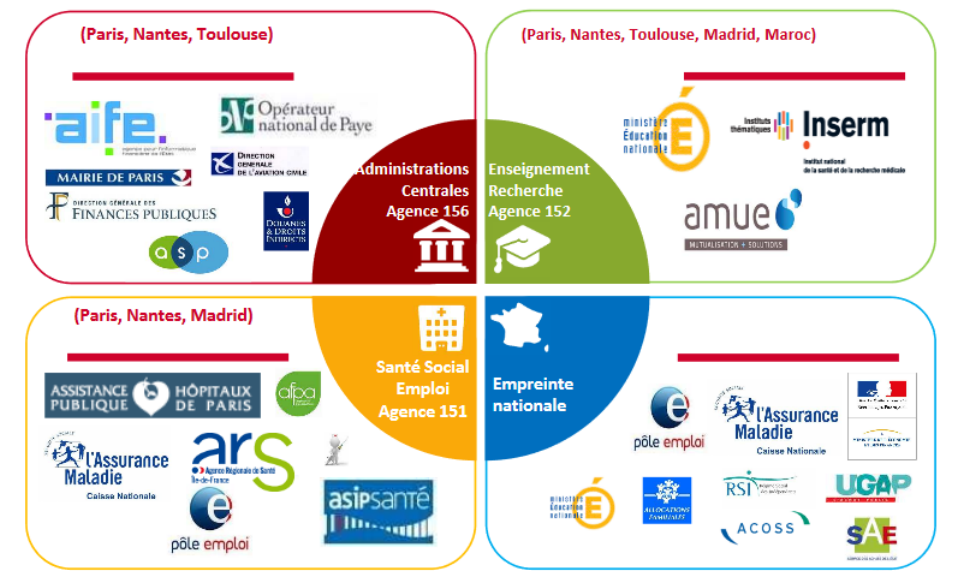
\includegraphics[width=1\textwidth]{images/divisionSecteurPublic.png}
\caption{Sopra Steria : Les agences du Secteur Public}
\end{figure}

\subsection{Focus sur l'agence 151 Santé Social Emploi}

L'agence 151 est répartie dans plusieurs villes : soit dans les locaux de Sopra Steria, soit directement chez le client.

Les projets sont pris en charge par des équipes. Une équipe peut travailler sur plusieurs projets simultanément, de même plusieurs équipes peuvent travailler sur un même projet. Les équipes sont généralement d’une dizaine de membres, parmi lesquels on retrouve les rôles de :
\begin{itemize}
    \item Chef de Projet (ou Project Manager),
    \item Analyste d’affaire (ou Business Analyst),
    \item Architecte,
    \item Expert produit (ou Product Expert),
    \item Solution Builder,
    \item Commercial.
\end{itemize}
\vspace{\baselineskip}
Mon équipe est installée avec d'autres équipes Sopra Steria dont le client est la CNAM. Nous sommes situés dans les locaux de Sopra Steria, tour Cytiscope à Montreuil. 

\section{Le client : la CNAM}

Chez Sopra Steria Group, plus de quatre cent collaborateurs travaillent pour le compte de la CNAM qui génère plus de 40 Millions d’euros de chiffre d’affaire. Ce chiffre est le plus important de toute la BU, ce qui fait de la CNAM un client d’importance maximale pour la société. Ce client gère les branches maladie du régime général de la sécurité sociale et représente :

\begin{itemize}
    \item 57 millions de bénéficiaires affiliés au régime général, 
    \item 4 assurés sur 5, 
    \item 75\% des dépenses de santé. 
\end{itemize}

Sopra Steria Group cherche à aider toutes ces entités en même temps dans leurs tâches quotidiennes. Les équipes de développement web (CNAM) travaillent pour atteindre ces objectifs. Je suis moi-même rattaché à la CNAM Métiers. Ci-dessous la liste des projets/équipes de la CNAM Métiers :

\begin{itemize}
    \item ARPEGE
    \item BIC : Briques I C
    \item CS Nantes
    \item DMP
    \item DPO
    \item DPRA
    \item INDIGO
    \item PPIL : Portail PILotage.
    \item OVERSI
\end{itemize}

\section{Le projet PPIL}

Cette partie aborde le projet PPIL, ses objectifs et ses fonctionnalités principales afin de donner une vue globale du projet.

\subsubsection{Un Portail de PILotage}

PPIL permet d'assurer le suivi des projets de la CNAM.
Celui-ci répond à plusieurs besoins :
\begin{itemize}
    \item Centralisation des informations de planification et de pilotage  au sein d’un même espace,
    \item Suivi et Contrôle grâce à des vues consolidées facilitant le suivi et la vérification des données de pilotage (actualisation des données, cohérence, …)
    \item Évolutivité et maintenance avec un socle qui permet de mettre en place de nouvelles fonctionnalités et de les déployer pour tous les utilisateurs,
    \item Faciliter la diffusion de l’information.
\end{itemize}
L'application PPIL a fait l'objet d'une refonte en 2017, désignée sous le nom PPIL V2. 
Le Portail Pilotage est composé de différents Espaces dont l’accès est conditionné par le profil de l’utilisateur. Les utilisateurs accèdent à leur espace et, selon leurs profils, les informations restituées à l’écran varient.

\subsubsection{Les utilisateurs de PPIL :}
PPIL comprend plusieurs types de profils, on peut citer tout d'abord les profils de type opérationnel, comprenant les : 
\begin{itemize}
    \item Responsable DSI
    \item MOA
    \item Managers (Responsable de Direction ou Responsable de Département) 
    \item Chef de Projet
\end{itemize}
Et on peut citer les profils de type stratégiques, comprenant les :
\begin{itemize}
    \item PMO
    \item Responsable de domaines
\end{itemize}
\vspace{\baselineskip}
Il ne faut pas oublier de citer les Visiteurs et Administrateurs.

\subsubsection{Les acteurs et leurs niveaux d'autorisation}
\begin{figure}[!h]
\centering
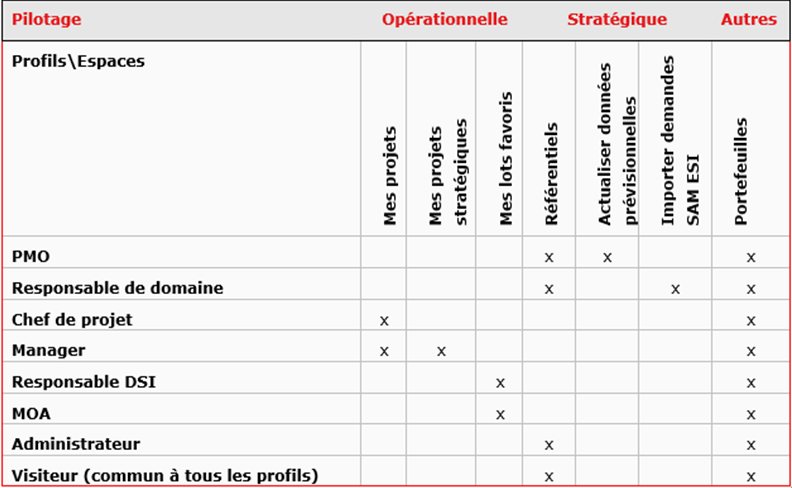
\includegraphics[width=0.8\textwidth]{images/ppil acteurs.png}
\caption{PPIL : Les acteurs et leurs autorisations}
\end{figure}

\subsubsection{Lien Lot - Projet - PRT Palier}

En bref, la CNAM a plein de projets qui groupé par lots. Les lots sont associé à un PRT Palier (division Métiers) et est constitué d'un projets de référence et de plusieurs projets contributeurs. Ci-dessous un schéma qui représente le lien entre entre ces entités.

\begin{figure}[!h]
\centering
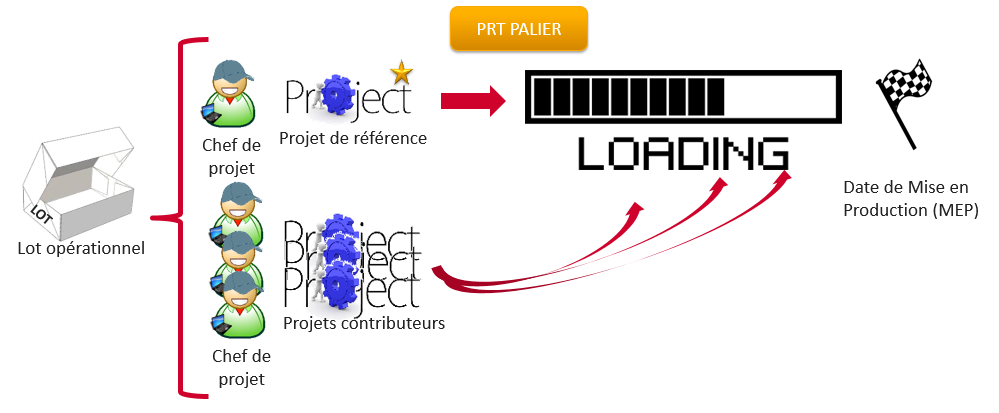
\includegraphics[width=0.9\textwidth]{images/ppil-lien-lot-projet-prtpalier.png}
\caption{PPIL : Lien lot projet PRT Palier}
\end{figure}

\subsubsection{Principe du Reporting - Suivi de projet}

Au sein de la CNAM, tous les acteurs d’un lot renseignent et mettent à jour le planning Microsoft Project(MSP) de leur projet, en renseignant des données du type :

\vspace{1\baselineskip}

\begin{itemize}
    \item Avancement charges, 
    \item Dates des jalons, 
    \item consommé des ressources.
\end{itemize}

\vspace{1\baselineskip}

Les informations MSP sont remontées dans PPIL de plusieurs manières :
\begin{itemize}
    \item Un batch automatique lancé 2 fois par jour
    \item Dans PPIL > Données prévisionnelles
    \item Dans PPIL > Actualiser les données MSP (Chef de Projet)
\end{itemize}

\vspace{1\baselineskip}

Tous les acteurs doivent renseigner les risques et problèmes rencontrés sur leur projet ainsi que l'état de leur projet.

\subsubsection{Principe du Reporting - Exemple du Chef de Projet}
Le CP du projet référent doit soumettre le reporting du lot toutes les 2 semaines (météo, tendance, situation).

Une fois soumis le reporting du lot est visible par tous les utilisateurs du portail.

Le Manager doit saisir la note de conjoncture du lot tous les 2 mois : cette action permet d'expliquer la situation opérationnelle du lot de manière moins technique, cette note de conjoncture est plus destiné aux supérieurs hiérarchiques (comme par exemple le Resp DSI).

\subsubsection{Chef de Projet}

Le Dashboard du CP comprend :

\begin{itemize}
    \item Bulletin de santé
    \item Dérive des jalons
    \item Plan de charges équipe
    \item Accès à la liste de mes projets en cours
    \item Note de conjoncture à mettre à jour
    \item Alertes
    \item Rapports
\end{itemize}

Ci-dessous l'accueil du CP :

\begin{figure}[!h]
\centering
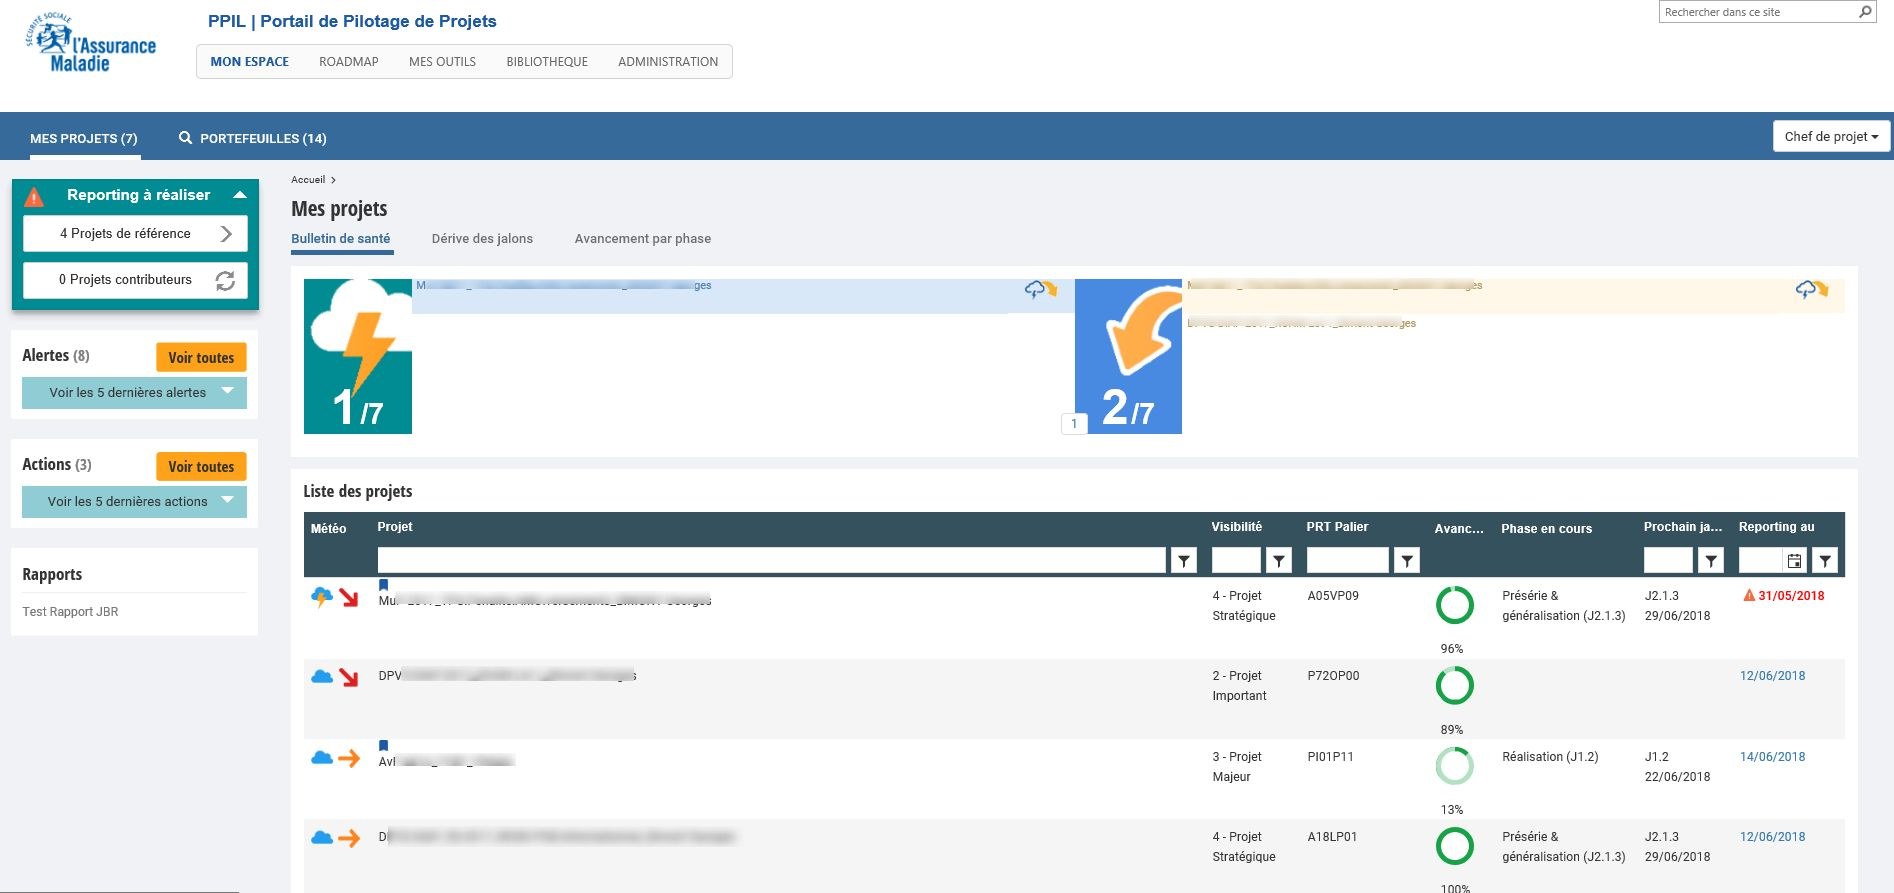
\includegraphics[width=1\textwidth]{images/ppil-CP-censored.png}}
\caption{PPIL : Accueil CP}
\end{figure}

Ci-dessous, un Chef de projet peut effectuer le reporting d'un projet :

\begin{figure}[!h]
\centering
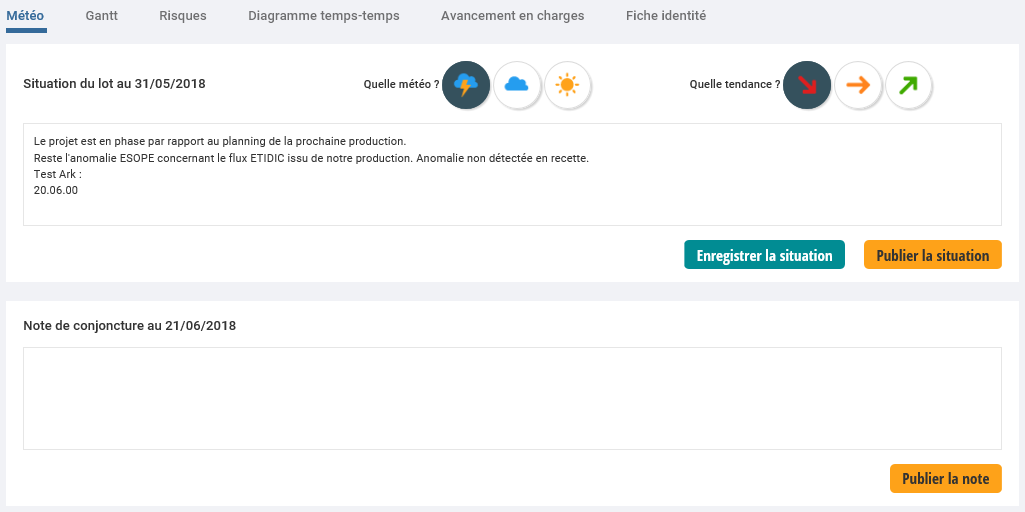
\includegraphics[width=1\textwidth]{images/ppil-meteo.PNG}
\caption{PPIL : Reporting et note de conjoncture}
\end{figure}

On peut aussi avoir accès au portail PPIL via une délégation.

%%% Local Variables: 
%%% mode: latex
%%% TeX-master: "isae-report-template"
%%% End: 